\documentclass[main.tex]{subfiles}

\begin{document}
        
\chapter{Marchés financiers}

\section{Historique}

La finance n'est pas un signe de modernité économique, les \textit{financial markets} existent depuis très longtemps. Ces derniers servent au début surtout à la négociation des effets publics, c'est dans la deuxième moitié du 19\up{ème} siècle qu'ils acquièrent un rôle plus important:
\begin{itemize}
        \item Décennie 1860 libération des sociétés par actions (SA)
        \item 1880 autorisation des marchés à terme, c'est à dire à découvert. 
\end{itemize}
Cet essor des marchés entraîne à la fin de cette période la deuxième révolution industrielle. On observe par la suite une décroissance de la place des marchés financiers, jusqu'à la fin des années 1970 ces derniers jouent un rôle secondaire, ce sont les banques qui financent l'économie. Un nouveau basculement vers les marchés capitaux se met en place avec les réformes majeures de la décennie 1980:
\begin{itemize}
        \item Acte unique européen sur la libre circulation des capitaux en 1986 
        \item Création d'Euronext en 2000 
\end{itemize}
Les marchés financiers reprennent leur place importante et détrônent les banques. Une nouvelle fois une fois l'essor des marchés financiers est accompagné d'une révolution industrielle, la troisième.

\begin{definition}[Euronext]
        Il s'agit de la principale place boursière de la zone euro avec plus de 1300 émetteurs représentant une capitalisation boursière totale de 3800 milliards d’euros. Son siège se trouve en France, le groupe est issue de la fusion des bourses de Paris Bruxelles et Amsterdam.
\end{definition}

\section{L'essor des marchés financiers}

\subsection{Les causes de cet essor\ldots}

On observe à la fin du 20\up{ème} siècle un essor important des marchés financiers aux États Unis, motivé par une politique économique forte souhaitant leur accorder une place principale au sein du capitalisme, quitte à surpasser celui des banques.
\begin{itemize}
        \item 1971: première fois que le dollar n'est plus indexé sur l'or, les réserves des États Unis s'épuisent. Cela induit d'importantes fluctuations dans le court des autres monnaies. Suite à cela de nouveaux produits financiers sont inventés pour contrer l'instabilité du SMI. Par example la création du premier marché de produits dérivés sur devises en 1972 à Chicago, moins d'un an après la fin des accords Bretton Woods.
        \item 1975: abolition progressive du \emph{Glass-Steagall Act} à Wall Street, les banques peuvent de nouveau être banque de dépôt et banque d'affaire. 
        \item 1979: nouvelle politique de la FED, mise en place par Paul Volcker, visant une hausse continue des taux d'intérêt pour stopper l'inflation. Les américains veulent accorder à l'économie de marché une place centrale au sein du capitalisme. Cette augmentation des taux d'intérêt, nominaux notamment, diminue les investissements et donc la consommation et l'inflation. Il s'agit d'une politique monétaire extrêmement brutale et sans précédent, ce même avant Reegan. Il s'en suit également une augmentation du chômage et une baisse de la croissance, on peine aujourd'hui  à manoeuvrer dans la direction opposée.
\end{itemize}

\begin{figure}[htpb]
        \centering
        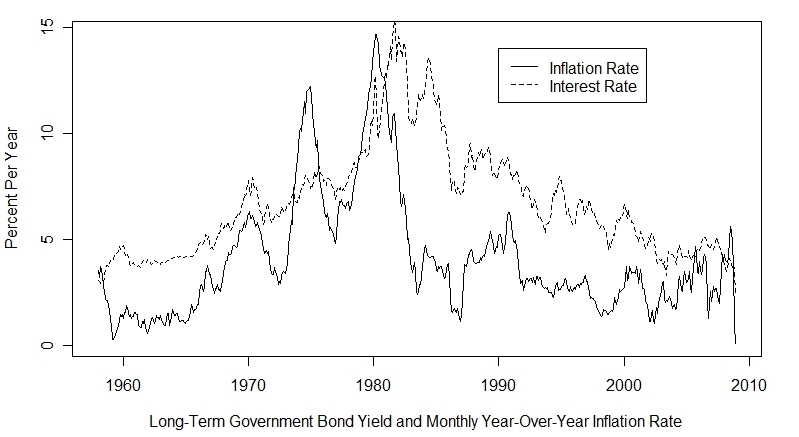
\includegraphics[width=0.8\textwidth]{interest_rates.jpg}
        \caption{Taux d'intérêt aux États Unis suite à la politique de la FED}
        \label{fig:interest_rates-jpg}
\end{figure}

On retrouve également ce \emph{Big Bang des marchés financiers} en Europe, notamment à Londres, avec la suppression des commissions de change en 1986, donnant l'autorisation aux marchés financiers étrangers d'acheter 100\% des actions des sociétés cotées britanniques. La City perd de son aspect nationaliste et s'ouvre d'avantage aux marchés internationaux.

\begin{definition}[Glass-Steagall Act]
        Adopté par le président Roosvelt en 1933, cet acte sépare les banques de commerce des banques d'investissement, ce afin de prévenir l'utilisation de l'épargne des utilisateurs pour investir sur des marchés financiers potentiellement risqués. Son abolition posera entre autres problème en 2008 lors de la crise des \emph{subprimes}. En France la Société Générale par exemple investit dans les subprimes avec le dépôt de ses utilisateurs. On discute alors la remise en place de cet accord sans succès.
\end{definition}

\subsection{\ldots et les conséquences}

Cet essor important des marchés financiers n'est pas sans conséquences. Si toutes sont à nuancer, certaines sont d'avantage positives et motivées par une comparaison à un système bancaire prédominant souffrant de certaines lacunes:
\begin{itemize}
        \item Une extension massive du rôle des marchés financiers favorise un gain théorique évident puisqu'ils sont considérés comme le système d'allocation des capitaux le plus efficient et le plus profond, permet la vente des produits à la valeur\ldots
        \item On juge qu'ils disposent d'une meilleure diffusion de l'information que les banques, pour être cotée en bourse une entreprise doit fournir un grand nombre d'informations qui sont vérifiées par divers acteurs
        \item Plus grande capacité à rendre liquides tous les actifs
        \item Meilleure répartition des risques, ceux ci sont toutefois \textit{`dilués'} sur un plus grand nombre de personnes qui en partageant donc les conséquences. Les risques peuvent avoir une répercussion plus grande et plus directe
\end{itemize}

D'autres conséquences le sont moins. Les marchés financiers sont beaucoup plus instables que les banques, ils ne fournissent pas les mêmes garanties et sont soumis à des régulations moins strictes:
\begin{itemize}
        \item Ils ne sont pas soumis aux réserves obligatoires, en général les règles qui les régulent sont plus faibles
        \item Ils ne bénéficient pas d'une appreciation rationnelle des risques, à l'inverse des banques, puisque les acteurs sont nombreux et plus diverses. Il est toutefois bon de noter que la crise des subprimes de 2008 a mis en évidence une mauvaise appréciation des risques de la part des banques, une limite à cette critique donc
        \item Ils ne bénéficient pas du rôle de \emph{prêteur en dernier ressort} des banques centrales qui ont le monopole d'émission. Une crise économique devenant une crise bancaire, les banques ont souvent eu recours à cet avantage, par exemple lors de la crise de 2019 des barils de pétrole en Arabie Saoudite. Notons que le paiement des créances par la banque centrale entraîne cependant une hausse du volume des liquidités et potentiellement une dépréciation de la monnaie, ce qui est peu souhaitable
\end{itemize}


Dans la même dynamique on observe aujourd'hui l'émergence de systèmes monétaires alternatifs comme le Bit coin qui s'affranchissent de la Banque centrale, mais ne bénéficient donc pas de la sécurité quelle peut offrir.


\subsection{Capitalisation boursière mondiale}

Les marchés financiers internationaux en concurrence directe permettent également de quantifier dans une certaine mesure le poids économique d'un pays ou d'une monnaie. On peut faire le lien avec le chapitre précédent en comparant une fois encore le dollar et l'euro, ou plus exactement les marchés américains et européens. Les États Unis représentent 50\% de la capitalisation boursière mondiale, l'Europe 20\% et 30 Tokyo, Zurich, Shanghai, Toronto et Hongkong se partagent la plus grande partie des 30\% restants. En chiffres, fin 2018 cela représente 23 billions dollars pour les États Unis, là où la City de Londres n'en pèse que 4,4 par exemple. Ceci illustre à nouveau la limite dans laquelle les objectifs économiques de l'Europe ont été atteints. \\
Enfin notons que les actif des investisseurs financiers représentent 150\% du PIB des États Unis, principalement des actions, et 100\% du PIB européen, surtout des obligations.


\section{La signification économique des variations d'un indice boursier, l'exemple du CAC 40}

\subsection{Quelques définitions}

\begin{definition}[Indice boursier]
        \emph{Share index} en anglais, il s'agit d'un indicateur clé pour déterminer la performance d'un marché. Les indices boursiers permettent aux investisseurs de gérer leur portefeuille d'actions. Ils sont représentatifs soit d'un marché, comme le \emph{CAC 40}, soit d'un secteur d'activité particulier tel que l'indice sectoriel de l'automobile.
\end{definition}

\begin{definition}[CAC 40]
        C'est un indice boursier qui prend en compte les 40 plus grosses sociétés françaises\footnote{Un comité se réunit pour mettre à jour la liste, cette dernière n'est pas exactement constituée des 40 sociétés les plus riches mais prend d'autres facteurs en compte.}, durablement installées dans une phase de croissance. Rétroactivement il augmente la visibilité des entreprises sur lesquelles il est indexé et donc les investissements, à l'inverse il n'est pas bon d'en sortir. Il est calculé comme une moyenne pondérée par la capitalisation des entreprises en function des titres boursiers qui circulent sur le marché. Il ne prend pas en compte les dividendes, souvent plus faible que les autres indices.
\end{definition}

\begin{definition}[CAC 40 \emph{gross return}]
       Il s'agit d'une version du CAC 40 qui intègre les dividendes dans son calcul, ce qui permet de le comparer aux autres indices qui les prennent également en compte. 
\end{definition}

\subsection{Interprétation de l'indice}

On serait tenter, à prime abord, d'interpréter les variations du CAC 40 comme une représentation de \textit{l'état de santé} des grandes entreprises françaises, et par extension du marché financier français puisque ces dernières représentent 75\% du PIB. \\

Il faut cependant différencier les secteurs, le luxe a tendance à tirer l'indice vers le haut tandis que d'autres secteurs vont moins bien. On peut comparer les actions de LVMH ou L'Oréal sur les 5 dernières années au secteur bancaire, notamment pour la société générale, ou au secteur industriel avec par exemple Renault dans l'industrie automobile. \\ 

Le CAC 40 semble de plus déconnecté de l'économie française, il ne reflète pas non plus l'évolution du taux de chômage ou de la croissance. Par exemple on constate une augmentation du CAC 40 entre 2012 et 2015 malgré une croissance presque nulle en France. On peut même supposer que les variations de cet indice représentent d'avantage l'état de l'économie internationale. Cela fait sens puisque les entreprises sur lesquelles il est indexé sont tournées vers le monde. Si de plus on compare le CAC 40 gross return, aux autres indices on ne peut s'empêcher de remarquer une tendance très similaire. 

\begin{figure}[htpb]
        \centering
        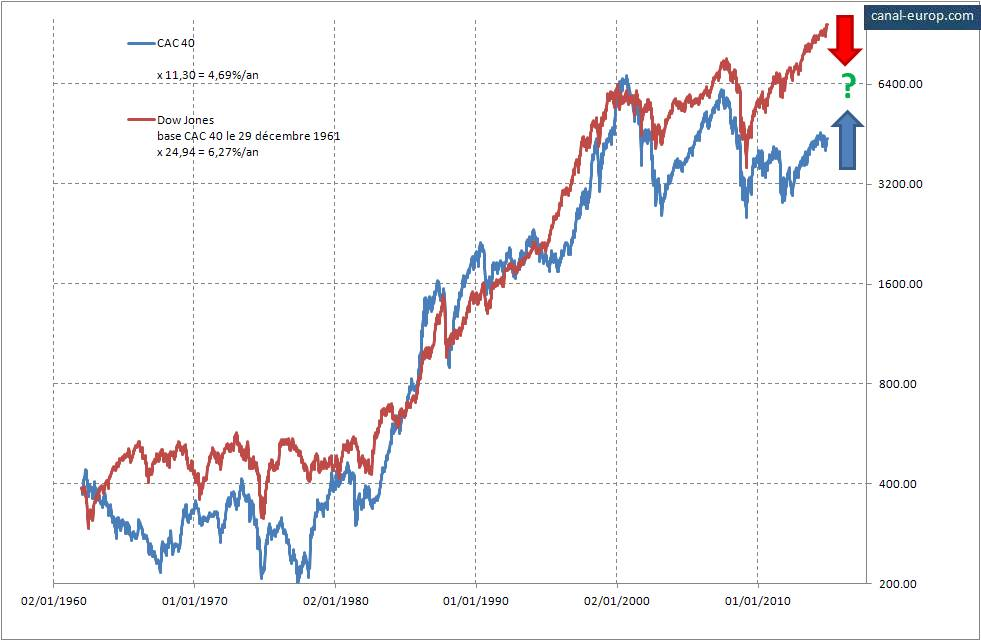
\includegraphics[width=0.8\textwidth]{CAC_DJ.jpg}
        \caption{Evolution du CAC 40 et du Dow Jones}
        \label{fig:CAC_DJ-jpg}
\end{figure}

Il est bon de noter que l'indice NASDAQ reste supérieur aux autres indices, ce qui traduit entre autres un manque d'entreprises dans le secteur de la haute technologie en France. En conclusion la hausse du CAC 40 reflète plus que l'économie internationale se porte bien. Les indices représentent une anticipation des investisseurs sur les marchés financiers.

\begin{definition}
        Le NASDAQ, \emph{National Association of Securities Dealers Automated Quotations} est une bourse de valeurs ouverte en 1971, parmi les plus important marchés d'actions des États-Unis en volume traité. Il est le plus grand marché électronique d'actions du monde, l'indice NASDAQ est l'indice boursier qui mesure la performance des entreprises qui y sont inscrites et cotées.
\end{definition}

\section{Analyser les variations boursières}

On se rend copte aujourd'hui qu'il est devenu très complexe, voire absurde, d'interpréter les variations boursières directement. Ces dernières sont étudiées, entre autres, comme marches aléatoires. Depuis le 20ème siècle de nombreuses preuves empiriques sont fournies sur le caractère aléatoire des variations des indices boursiers, comme c'est le cas par exemple pour le Dow Jones.
En toute logique il est devenu impossible de prévoir les cours à venir. Seule la variabilité instantanée peut l'être, la réalité est trop instable et évolue trop rapidement pour permettre la formalisation d'un modèle prédictif efficace.

\subsection{La notion d'efficience informationnelle}
Si on ne peut modéliser les variations boursière, l'information disponible et les moyens amenant à son obtention jouent néanmoins un rôle primordial dans l'élaboration des plans de placement. 

\begin{definition}[Efficience informationnelle]
        Le concept est inventé par Paul Samuelson puis Eugène Fama, ce dernier définit le terme dans une publication du \textit{Journal of Science} en 1970. Selon lui \textit{`un marché informationnellement efficient est défini comme étant un marché sur lequel le prix observé reflète pleinement et instantanément toute l'information disponible'}. Un tel marché incorpore donc instantanément les conséquences des évènements passés et reflète avec précision les anticipations exprimées sur les évènements futurs. Un tel marché suppose de plus une allocation optimale des ressources disponibles. Selon cette théorie il n'y a \textbf{pas} d'auto corrélation des prix. Chaque agent participant au marché interprète individuellement l'information disponible, égale pour tous, et tous convergent vers la même estimation de la \emph{valeur fondamentale}.
\end{definition}

\begin{definition}[Valeur fondamentale]
        Valeur objective des marchandises et des actions d'une entreprise basée sur la quantité de travail utile à la production des marchandises.
\end{definition}
        
\subsection{Critique de l'efficience informationnelle}

Il existe deux critiques internes majeurs concernant l'efficience informationnelle
\begin{itemize}
        \item Le paradoxe de Grossman et Stiglitz, l'hypothèse d'autoréférentialité, \textit{On the impossibility of informationally efficient markets}
        \item La critique de Schiller: la variance des dividendes est beaucoup plus faible que celle du cours des actions, \textit{The volatility of stock market prices}
\end{itemize}

\subsection{Trois courants d'analyse}

\begin{itemize}
        \item Néoclassiques orthodoxes Fama valeur fondamentale et efficience informationnelle
        \item Néoclassiques critiques Shiller, Schleifer \textit{noise trader approach}, volatilité et imprévisibilité des marchés, \textit{narrative economics} et autorérentialité
        \item Théorie mimétique Keynes, rôle central de l'intersubjectivité et du mimétisme, exemple du concours de beauté
\end{itemize}

\section{Agences de notation}

\subsection{Définitions et exemples, un oligopole américain}

\begin{definition}[Agence de notation]
        \emph{Credit Rating Agency} en anglais, c'est un organisme chargé d'évaluer le risque de non-remboursement de la dette ou d'un emprunt d'un État, d'une entreprise ou d'une collectivité locale, \textit{etc.} Rémunérée par le demandeur de notation financière, elle produit, à titre indicatif, des outils qui estiment les risques d'insolvabilité. Différentes échelles de notation existent suivant les agences, les entités notées et la période considérée, long terme ou court terme. 
\end{definition}

Les trois principales agences de notation sont aujourd'hui \emph{Goody's, Standard \& Poors} et \emph{Fitch Ratings}. Ces trois entreprises  américaines détiennent à elles seules plus de 85\% du marché, il s'agit d'un véritable oligopole américain.  Ce dernier pose le problème de l'autorenforcement. Les entreprises souhaitent être notées par les agences les plus réputées, ce qui a pour effet secondaire de renforcer la popularité de ces agences. Il est bon de noter que ces agences sont juges et parti. Le processus de \emph{rating} devient alors itératif, l'agence conseillant le structureur, celui-ci soumet une proposition, si l'objectif de \emph{rating} n'est pas atteint il revoit sa copie ou va voir une autre agence. On voit alors nettement à quel conflit d'intérêts les agences sont confrontées, et il n'est pas surprenant que certaines aient cédé à une certaine complaisance vis-à-vis de leurs clients qui sont, ceux-là même qu'elles sont censées noter. Pire, ces derniers ne les paieront que si le \emph{rating} est finalement publié, ce qui leur procure un levier supplémentaire. Cela met en évidence une seconde critique de cet oligopole et nous amène à la deuxième section.

\subsection{Une critique du système actuel}

Les notes émises par les agences de notation ont une répercussion directe et puissante sur l'économie de grandes institutions, leurs décisions peuvent induire un bouleversement social économique et politique au sein même d'un pays. \\
Malgré cela les agences insistent beaucoup sur le fait que le \emph{rating} représente une opinion, et non une quelconque forme de garantie ou d'engagement de leur part, ce qui au regard de la loi américaine les met à l'abri de poursuites de la part des investisseurs. Le \emph{rating} a ses limites, il constitue une évaluation du risque de crédit à l'exclusion de tout autre risque. Il ne donne aucune indication sur la rentabilité potentielle d'un investissement, ni sur la volatilité des titres émis.

\begin{itemize}
        \item En 1931 \emph{Moody's} dégrade la Grèce, les problèmes économiques qui en découlent sont suivis d'émeutes, la monarchie est rétablie puis renversée par un coup d'état en 1936. En 2009 la Grèce descend de 9 critères dans l'échelle de notation, ce qui prolonge et empire la crise économique du pays
        \item Les erreurs parfois coûteuses des agences de notation amènent une perte de confiance en ces dernières. L'affaire Eron est un bon exemple, une entreprise notée AAA, la meilleure note, jusqu'à 3 jours avant sa faillite. La société empruntait à l'aide d'autres sociétés écran pour cacher ses dettes, les agences ont pu être bernées par des manipulations comptables
        \item Les agences manquent parfois de recul, ce fut le cas lors des \emph{subprimes}, les prêts à des usagers peu solvables étaient notés AAA aussi, les agences n'ont pas vu la crise venir
\end{itemize}

En réponse à cela, l'Europe a mis en place la création d'une certification européenne sur les agences de notation qui y exercent, applicable à partir d'avril 2010. Ce règlement prévoit une procédure d'enregistrement des agences auprès du \emph{Committee of European Securities Regulators}, devenu l'ESMA, l'obligation d'une plus grande transparence sur les méthodes utilisées, la façon dont les conflits d'intérêt sont gérés, \textit{etc.} En parallèle des agences de notation sociétales se développent ainsi qu'un système de notation interne.
\end{document}
